%---------------------------------------------------------------------
%
%                          Proteopathogen 1
%
%---------------------------------------------------------------------

\begin{otherlanguage}{british}

\chapter*{\href{http://www.ncbi.nlm.nih.gov/pubmed/19743419}{Proteopathogen, a protein database for studying \mbox{\textit{Candida albicans}} - host interaction}}

\addcontentsline{toc}{chapter}{Proteopathogen, \\  a protein database for studying \textit{Candida albicans} - host interaction}
%\fancyhf{} % clear all header and footer fields
%\restauraCabecera
\fancyhead[RO,LE]{\sc{Proteopathogen, a protein database for studying \mbox{\textit{Candida albicans}} - host interaction}}


\addcontentsline{lof}{chapter}{Proteopathogen, \\  a protein database for studying \textit{Candida albicans} - host interaction}
\addcontentsline{lot}{chapter}{Proteopathogen, \\  a protein database for studying \textit{Candida albicans} - host interaction}



%\renewcommand{\headrulewidth}{0pt}
\cabeceraEspecial{Proteopathogen database to study \textit{\mbox{C. albicans}} - host interaction}

\subsubsection*{Vital Vial\'as, Rub\'en Nogales-Cadenas, C\'esar Nombela, Alberto Pascual-Montano, \mbox{Concha Gil}}
\subsubsection*{Proteomics 2009, 9, 4664-4668}



\bigskip
\hfill
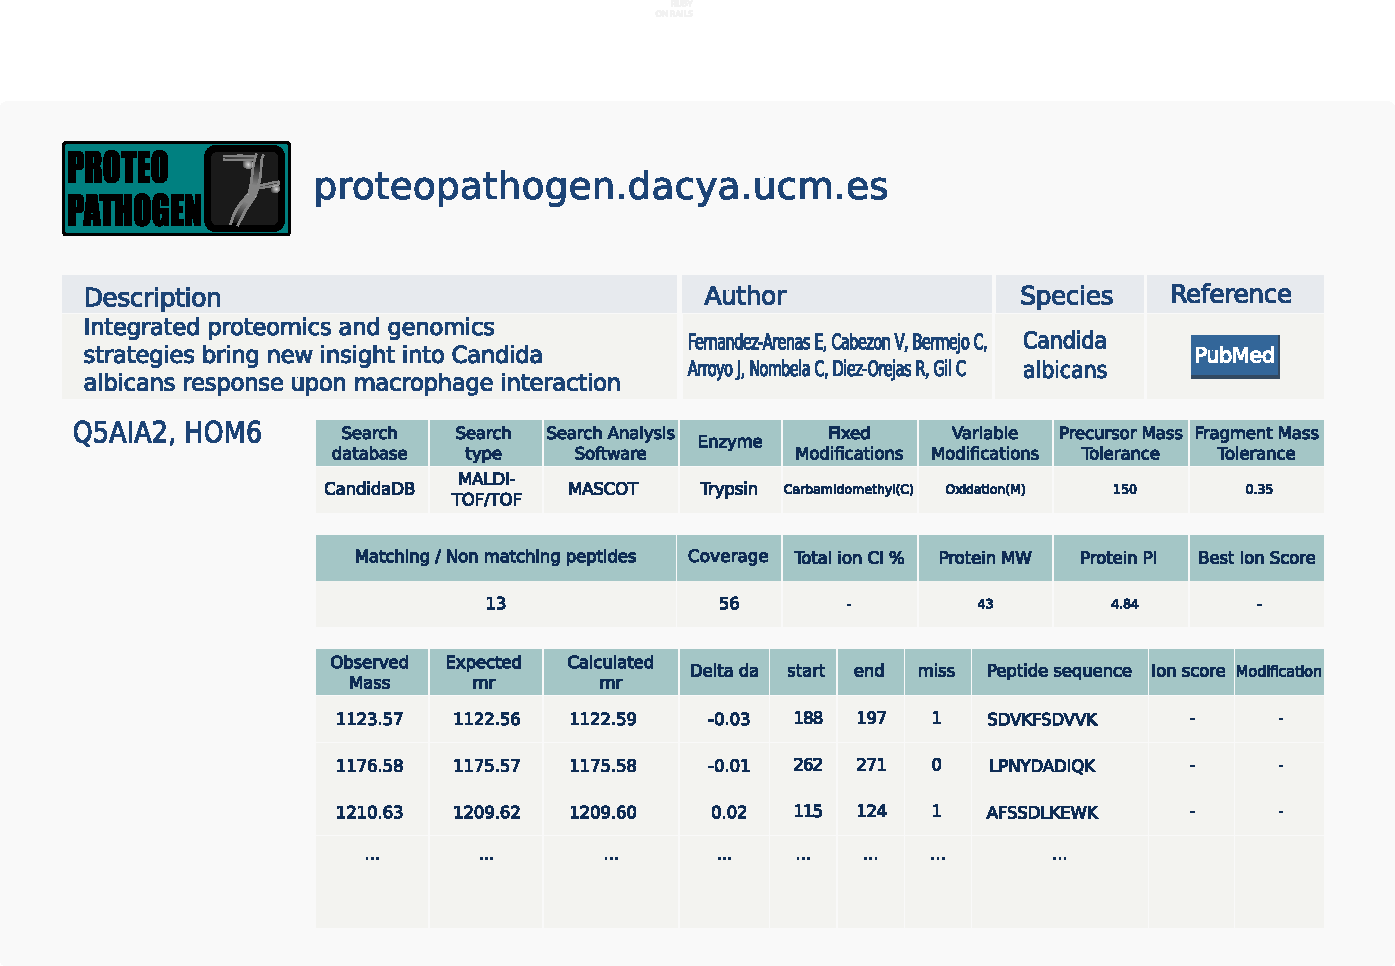
\includegraphics[width=1\textwidth]{Imagenes/Vectorial/graphical_abstract_Proteopathogen1}



\newpage

%\includepdf[pages=-,scale=.85,pagecommand={}]{Capitulos/Vialas_2009_Proteopathogen_Proteomics.pdf}
%\includepdf[pages=-,pagecommand={}]{Proteopathogen/Vialas_2009_Proteopathogen_Proteomics.pdf}


%\section*{Proteopathogen, a protein database for studying \mbox{\textit{Candida albicans}} - host interaction}

\chapter*{Abstract}

There exist, at present, public web repositories for management and storage of proteomic
data and also fungi-specific databases. None of them, however, is focused to the specific
research area of fungal pathogens and their interactions with the host, and contains
proteomics experimental data. In this context, we present Proteopathogen, a database
intended to compile proteomics experimental data and to facilitate storage and access to a
range of data which spans proteomics workflows from description of the experimental
approaches leading to sample preparation to MS settings and peptides supporting protein
identification. Proteopathogen is currently focused on \textit{Candida albicans} and its interaction
with macrophages; however, data from experiments concerning different pathogenic fungi
species and other mammalian cells may also be found suitable for inclusion into the database. 

Proteopathogen is publicly available at \href{http://proteopathogen.dacya.ucm.es}{http://proteopathogen.dacya.ucm.es}

\newpage{}

\textit{Candida albicans} is an opportunistic pathogenic fungus,
which can be found as a component of the usual flora in
human mucoses. Although it does not normally cause
disease in immunocompetent colonized hosts, in the case
of immunosuppressed patients \textit{Candida} cells can overproliferate
 and become pathogenic. Cells in yeast form (oval
cells) may produce hyphae, penetrate tissues and eventually
cause invasive candidiasis. At present, the frequency of this
fatal opportunistic mycosis continues to be distressing and,
unfortunately, solution is hindered by the reduced effectiveness
 and serious side effects of the few available drugs,
the appearance of antifungal-drug resistance, and the lack of
accurate and prompt diagnostic procedures \citep{Calderone2012}.

Addressing proteomic studies involving the way \textit{Candida}
interacts with immune cells is thus essential in order to
improve our comprehension of the process of infection and
represents the primary step of investigation that could lead
to future development of diagnosis methods, vaccines and
antifungal drugs \citep{Fernandez-Arenas2007, Martinez-Solano2006a, Pitarch2006, Pitarch2006a}.


Experimental techniques in proteomics have quickly
evolved in such a way that nowadays we have to deal with
vast amounts of complex data originated by the combination
of multi-dimensional separation techniques and MS analysis
 together with the bioinformatics software reports \citep{Monteoliva2004}.
Existing public repositories for management and storage of
proteomic data such as World 2-D PAGE \citep{Hoogland2008}, the Proteome
Database System for Microbial Research 2-D PAGE \citep{Pleissner2004}, or
PRIDE \citep{Martens2005}; and fungi-specific databases such as BioBase
MycoPathPD \citep{Csank2002}, Candida Genome Database (CGD) \citep{Arnaud2005}
or Candida DB \citep{Rossignol2008} are very popular and useful tools.
However, none of them deals with proteomic experimental
data related to the specific research area of fungal pathogens
and their interaction with the host. In this context,
we present Proteopathogen, a protein database, currently
focused on the \textit{\mbox{C. albicans}} - macrophage interaction
model - which enables a framework for the access and
submission of proteomic workflow data, from description of
the experimental approaches leading to sample preparation
to MS settings and identification - supporting peptides.
Through its interface web site, the database can easily be
queried to allow an efficient browsing through all the stored
data, improving the quality of eventual analysis of MS
results.

Regarding the compilation of information used to
populate the database, data from three different studies were
considered suitable to be present in Proteopathogen.
The first two correspond to publish works relating to
proteomics of the \textit{Candida} - macrophage interaction
\citep{Fernandez-Arenas2007, Martinez-Solano2006a}, where the former reports 
66 different \textit{\mbox{C. albicans}}
identified proteins and the latter, 38 murine macrophage
proteins. The third study represents an analysis of the
\textit{\mbox{C. albicans}} plasma membrane proteome \citep{Cabezon2009}. It compiles
a set of experiments aimed at extraction and identification of
membrane proteins and a set of experiments intended to
obtain enrichment in glycosylphosphatidylinositol-anchored
surface proteins, which have been reported to be involved in
cell wall biogenesis, cell-cell adhesion and interaction with
the host \citep{Plaine2008}.




\begin{table}[t]

\caption*{Table 1. Overview of the stored data in Proteopathogen as well as their published evidences.}

\renewcommand{\arraystretch}{2}
\footnotesize
\centering

\begin{tabular}{p{3cm} p{4cm} l p{2cm} }

\hline
References & Description of  \newline{} experimental approach & Species & \#Protein \newline{} identifications \\
\hline
\

\citep{Fernandez-Arenas2007} & \mbox{C. albicans} differentially expressed proteins after 3 h interaction with RAW 264.7 murine macrophages. 2-D silver-stained gel. MS/MS (MALDI/TOF-TOF) & \textit{\mbox{C. albicans}} & 66\\

\citep{Martinez-Solano2006a} & Proteins identified from cytoplasmic extracts of RAW 264.7 cells after 45 min interaction with \textit{C.albicans} & \textit{Mus musculus} & 38\\

\citep{Cabezon2009} & Identification of Glycosyl phosphatidil inositol (GPI)-anchored membrane proteins & \textit{C. albicans} & 292\\

 & Identification of membrane proteins &  & 1273\\

\end{tabular}
\end{table}
\addcontentsline{lot}{table}{Table 1}



In all cases, protein identifications lists are collected
together with the pertinent experimental context specified
by descriptions of the experimental approaches, MS settings
and peptides supporting identification for each of the
proteins (Table 1).

Along with the experimental information, and in order to
provide a deeper view of the data, complementary information
 is retrieved from public web repositories. In the
case of \textit{\mbox{C. albicans}} proteins, identifiers, synonyms, aminoacid
sequence of the translated open reading frame, \textit{Saccharomyces
cerevisiae} orthologs, Gene Ontology (GO) annotation, pathway
annotations and scientific literature references were obtained
from CGD \citep{Arnaud2005}, whereas in the case of murine macrophage
proteins, the equivalent information was obtained from
UniProt KnowledgeBase \citep{Uniprot2008} and the Mouse Genome Database
 \citep{Bult2008}. Additionally, pathways annotations were retrieved
from Kyoto Encyclopedia of Genes and Genomes (KEGG)
Pathway Database \citep{Kanehisa2007} and structure information from the
Protein Data Bank (PDB) \citep{Berman2000}.

\setcounter{chapter}{2}
\setcounter{figure}{0}

%\figura{Vectorial/proteopathogen1}{width=.99\textwidth}{fig:proteopathogen1}%
%{Search for \textit{C. albicans} ubiquinol-cytochrome-c reductase QCR2}



\begin{figure}[t]
\begin{center}
 \includegraphics[width=0.99\textwidth]%
				 {Imagenes/Vectorial/proteopathogen1}
\caption*{Figure 1. Use case: Search for \textit{\mbox{C. albicans}} ubiquinol-cytochrome-c
reductase QCR2. The different sections in the result comprise information
on protein description and identifiers, experiments in which it has been
identified, GO annotation, KEGG and CGD pathway annotation and 
structural information from PDB.}
\end{center}
\end{figure}
\addcontentsline{lof}{figure}{Figure 1}

Concerning the architecture of the software, the back-end
layer consists of a MySQL database managed by the web
application development framework Ruby on Rails that sets
up structure and relations of data, handles queries to the
database and displays the user web-based interface.

The experimental context is addressed in Proteopathogen
in a hierarchical manner, where a main general approach,
which may correspond to a published article, is characterized
 by a description or title, authors, target species and
Pubmed identifier when available; and experiments within
it, are in they turn, characterized by the description of the
particular experiment, the date when it was performed and
number of identified proteins.

Information on one particular protein is split into several
sections in Proteopathogen. Protein Basic Information
displays the UniProt accession number, description, species,
evidence for the existence, standard gene name, organism-
specific database identifiers, yeast orthologs for \textit{Candida}
proteins and human orthologs for mouse proteins and
sequence. The Section 2 lists experiments in which the
particular protein has been identified. Where available,
one or more of the following sections will be displayed
as well: the table entitled GO showing GO annotations
along with the pertinent scientific references, the KEGG
Pathways and CGD Pathways tables rendering annotations
from KEGG and CGD respectively, and PDB, a table
specifying structural information. Where no PDB identifiers
are found for \textit{\mbox{C. albicans}} proteins, \textit{S. cerevisiae} orthologs
are used instead, and similarly, when a PDB identifier
cannot be found for mouse proteins, the human ortholog
is used.

In all cases, proteins are unambiguously related to their
corresponding experiment, thus enabling a relation to the
data concerning experimental parameters of identification
and identification-supporting peptides. This data comprise,
on the one hand, common MS settings for all proteins
identified in the particular experiment, including search
database, MS type, analysis software, digestion enzyme,
fixed aminoacid modifications, variable modifications and
maximum allowed number of miscleavages; and on the
other hand, particular parameters and peptides list for each
protein, including number of matched peptides, score,
observed peptide mass, calculated peptide mass, start and
end coordinates, number of missed cleavages and the
sequence of the peptide.

The web interface to Proteopathogen offers multiple
ways to query the database. Through the Browse Experiments
search option, a list containing all sets of experimental
approaches is displayed. In its turn, one particular
experiment can be browsed through all the proteins
identified in it.

The Search form may be used in different manners.
Queries for one particular protein can be performed by
supplying one of the multiple supported identifiers, namely
standard gene names, \textit{Candida} feature name, Candida DB
identifiers, CGD identifiers, MGI identifiers and UniProt
accession numbers. Free text queries can be performed as
well, which will retrieve a list of proteins showing coincidences
 in the description field of the Proteopathogen
protein entry. As an additional feature, peptide sequences
can also be searched for retrieving in this case, proteins in
any experiment having the searched sequence in any of the
identification-supporting peptides. Wild characters (*)
and boolean operators are supported for free text queries
and for peptide sequence queries.

In order to enhance interactivity and collaboration
with users, a submission form is included in the web
interface to allow the upload of more proteomic experimental
 approaches as long as they concern the topics
addressed in Proteopathogen. Sequential steps request from
the user the following information: a description of the
experimental context, a related protein list, MS parameters
and identification-supporting peptides lists. These data are
subject to revision prior to eventual insertion into Proteo-
pathogen by the database curators. Besides, the whole relational
 database and the MS data reports are available for
download at the web site.

All the information that is retrievable from Proteo-
pathogen when queried for one particular protein is shown
in Fig. 1 for the specific case of ubiquinol-cytochrome-c
reductase QCR2 of \textit{\mbox{C. albicans}} which has been reported to
show antigenic properties in human \citep{Pitarch2004}.

The Protein Basic Information section displays the
Uniprot accession number, a brief description of the protein
as stated at CGD, evidence for its existence, standard gene
name, feature name, CGD and Candida Database identi-
fiers, yeast ortholog gene name, synonyms and sequence.

The Section 2 lists all the experiments in which QCR2
has been identified. All of them belong to the same general
approach aimed at purification of membrane proteins. In
every case, the corresponding links to the MS identification
parameters and supporting peptides are displayed as well.
This experimental data are shown in Fig. 1 for identification
of QCR2 in the experiment described as "Method D.
Douncer homogenizer protoplast breaking and 12-60%
sucrose gradient. LC-LTQ".

The section entitled GO annotations shows terms related
to the electron transport chain, but more interestingly, it
also shows an inferred from direct assay (IDA) annotation to
the term membrane fraction \citep{Insenser2006}, which fits to the fact that
the protein is identified in five of the methods aimed at
purification of membrane proteins.

KEGG Pathways table provides a link to the KEGG
Pathway entry for Oxidative phosphorylation, and provides
the feature to show in place the image corresponding to the
map from KEGG. CGD Pathways displays an analogous link
to the pathway entry at CGD that, in this case, is named
aerobic respiration (cyanide sensitive)- electron donors.

Finally, in the PDB section, there are four structure
images available along with links to the PDB entries,
corresponding to a cytochrome bc1 complex from \textit{S. cerevisiae}.
 Orthologs were used since no structure could be found
for the \textit{Candida} protein.

In conclusion, Proteopathogen represents, up to date, the
first public web-based repository for proteomics data related
to studies involving \textit{\mbox{C. albicans}} pathogenicity and its interaction
 with immune system cells in the host. Moreover, it
enables a framework for public access and submission of
this type of data and it is intended to be more actively
populated in the near future, including data from different
pathogenic fungi and mammalian cells, becoming a refer-
ence database in its field. Unlike other protein identification
databases, Proteopathogen is focused to a specific topic but,
at the same time, includes a wide range of data including
descriptions of the experimental contexts, information on
proteins such as GO and pathway annotations, structural
information and detailed MS parameters. Therefore,
Proteopathogen will contribute to save time and facilitate
analysis of proteomic workflow reports for researchers
interested in this area.

\medskip

\textit{
The authors are grateful to C\'esar Vicente from the Computer
Architecture Department, Complutense University of Madrid for
his excellent technical assistance. This work was supported by
BIO 01989-2006 from the Comision Interministerial de Ciencia
y Tecnolog\'ia (CYCIT, Spain), DEREMICROBIANA - CM
from Comunidad Autonoma de Madrid, and REIPI, Spanish
Network for the Research in Infectious Diseases, RD06/0008/
1027 from the Instituto de Salud Carlos III. The Proteomics
work was carried out in the Proteomics Unit UCM-Parque
Cient\'ifico, a member of the National Institute for Proteomics
PROTEORED, funded by Genoma Espa\~na. APM and RNC are
partially supported by Spanish grants BIO2007-67150-C03-02,
S-Gen-0166/2006 and PS-010000-2008-1.
The authors have declared no conflict of interest.
}


\section*{References}


\begin{itemize}[leftmargin=*]

\item[]{
Arnaud, M. B., Costanzo, M. C., Skrzypek, M. S., Binkley, G., Lane, C., Miyasato, S. R., and
Sherlock, G. (2005), The Candida Genome Database (CGD), a community resource for
\textit{Candida albicans} gene and protein information., Nucleic acids research, 33(Database issue), D358-63.
}

\item[]{
Berman, H. M., Westbrook, J., Feng, Z., Gilliland, G., Bhat, T. N., Weissig, H., Shindyalov, I. N.,
and Bourne, P. E. (2000), The Protein Data Bank., Nucleic acids research, 28(1), 235-42.
}

\item[]{
Bult, C. J., Eppig, J. T., Kadin, J. A., Richardson, J. E., and Blake, J. A. (2008), The Mouse
Genome Database (MGD): mouse biology and model systems., Nucleic acids research,
36(Database issue), D724-8.
}

\item[]{
Cabez\'on, V., Llama-Palacios, A., Nombela, C., Monteoliva, L., and Gil, C. (2009), Analysis of
\textit{Candida albicans} plasma membrane proteome., Proteomics, 9(20), 4770-86.
}

\item[]{
Calderone, R. (2012), Candida and candidiasis. ASM Press, Washington DC.
}

\item[]{
Csank, C., Costanzo, M. C., Hirschman, J., Hodges, P., Kranz, J. E., Mangan, M., O'Neill,
K., Robertson, L. S., Skrzypek, M. S., Brooks, J., and Garrels, J. I. (2002), Three yeast
proteome databases: YPD, PombePD, and CalPD (MycoPathPD)., Methods in enzymology,
350, 347-73.
}

\item[]{
Fern\'andez-Arenas, E., Cabez\'on, V., Bermejo, C., Arroyo, J., Nombela, C., Diez-Orejas, R.,
and Gil, C. (2007), Integrated proteomics and genomics strategies bring new insight into
\textit{Candida albicans} response upon macrophage interaction, Molecular \& cellular proteomics
: MCP, 6(3), 460-478.
}

\item[]{
Hoogland, C., Mostaguir, K., Appel, R. D., and Lisacek, F. (2008), The World-2DPAGE 
Constellation to promote and publish gel-based proteomics data through the ExPASy server.,
Journal of proteomics, 71(2), 245-8.
}

\item[]{
Insenser, M., Nombela, C., Molero, G., and Gil, C. (2006), Proteomic analysis of detergent -
resistant membranes from Candida albicans., Proteomics, 6 Suppl 1, S74-81.
}

\item[]{
Kanehisa, M., Araki, M., Goto, S., Hattori, M., Hirakawa, M., Itoh, M., Katayama, T., 
Kawashima, S., Okuda, S., Tokimatsu, T., and Yamanishi, Y. (2007), KEGG for linking genomes to
life and the environment, Nucleic Acids Research, 36(Database), D480-D484.
}

\item[]{
Martens, L., Hermjakob, H., Jones, P., Adamski, M., Taylor, C., States, D., Gevaert, K., Van-
dekerckhove, J., and Apweiler, R. (2005), PRIDE: the proteomics identifications database.,
Proteomics, 5(13), 3537-45.
}

\item[]{
Mart\'inez-Solano, L., Nombela, C., Molero, G., and Gil, C. (2006), Differential 
protein expression of murine macrophages upon interaction with \textit{Candida albicans}, Proteomics, 6 Suppl
1, S133-S144.
}

\item[]{
Monteoliva, L. and Albar, J. P. (2004), Differential proteomics: an overview of gel and non-gel
based approaches., Briefings in functional genomics \& proteomics, 3(3), 220-39.
}

\item[]{
Pitarch, A., Abian, J., Carrascal, M., S\'anchez, M., Nombela, C., and Gil, C. (2004),
Proteomics-based identification of novel \textit{Candida albicans} antigens for diagnosis 
of systemic candidiasis in patients with underlying hematological malignancies.,
Proteomics, 4(10), 3084-106.
}

\item[]{
Pitarch, A., Nombela, C., and Gil, C. (2006a), \textit{Candida albicans} biology and pathogenicity:
insights from proteomics., Methods of biochemical analysis, 49, 285-330.
}

\item[]{
Pitarch, A., Nombela, C., and Gil, C. (2006b), Contributions of proteomics to diagnosis, treat-
ment, and prevention of candidiasis., Methods of biochemical analysis, 49, 331-61.
}

\item[]{
Plaine, A., Walker, L., Da Costa, G., Mora-Montes, H. M., McKinnon, A., Gow, N. A. R., 
Gaillardin, C., Munro, C. A., and Richard, M. L. (2008), Functional analysis of Candida albicans
GPI-anchored proteins: roles in cell wall integrity and caspofungin sensitivity., 
Fungal genetics and biology : FG \& B, 45(10), 1404-14.
}

\item[]{
Pleissner, K.-P., Eifert, T., Buettner, S., Schmidt, F., Boehme, M., Meyer, T. F., Kaufmann, S.
H. E., and Jungblut, P. R. (2004), Web-accessible proteome databases for microbial 
research., Proteomics, 4(5), 1305-13.
}

\item[]{
Rossignol, T., Lechat, P., Cuomo, C., Zeng, Q., Moszer, I., and D'Enfert, C. (2008), 
CandidaDB: a multi-genome database for Candida species and related Saccharomycotina.,
Nucleic acids research, 36(Database issue), D557-61.
}

\item[]{
The Uniprot Consortium (2008), The universal protein resource (UniProt).,
Nucleic acids research, 36(Database issue), D190-5.
}

\end{itemize}




%~ \setBibFiles{proteopathogen1}
%~ 
%~ \def\ficherosBibliografia{}
%~ \newcommand{\setBibFiles}[1]{
%~ \def\ficherosBibliografia{#1}
%~ }
%~ 
%~ \begingroup
%~ \spanishdeactivate{~}
%~ \bibliographystyle{TeXiS/TeXiS}
%~ %\bibliographystyle{abbrv}
%~ \bibliography{\ficherosBibliografia}
%~ \endgroup


\end{otherlanguage}